 \section{Setup}


  \begin{figure}[h!]
    \centering
    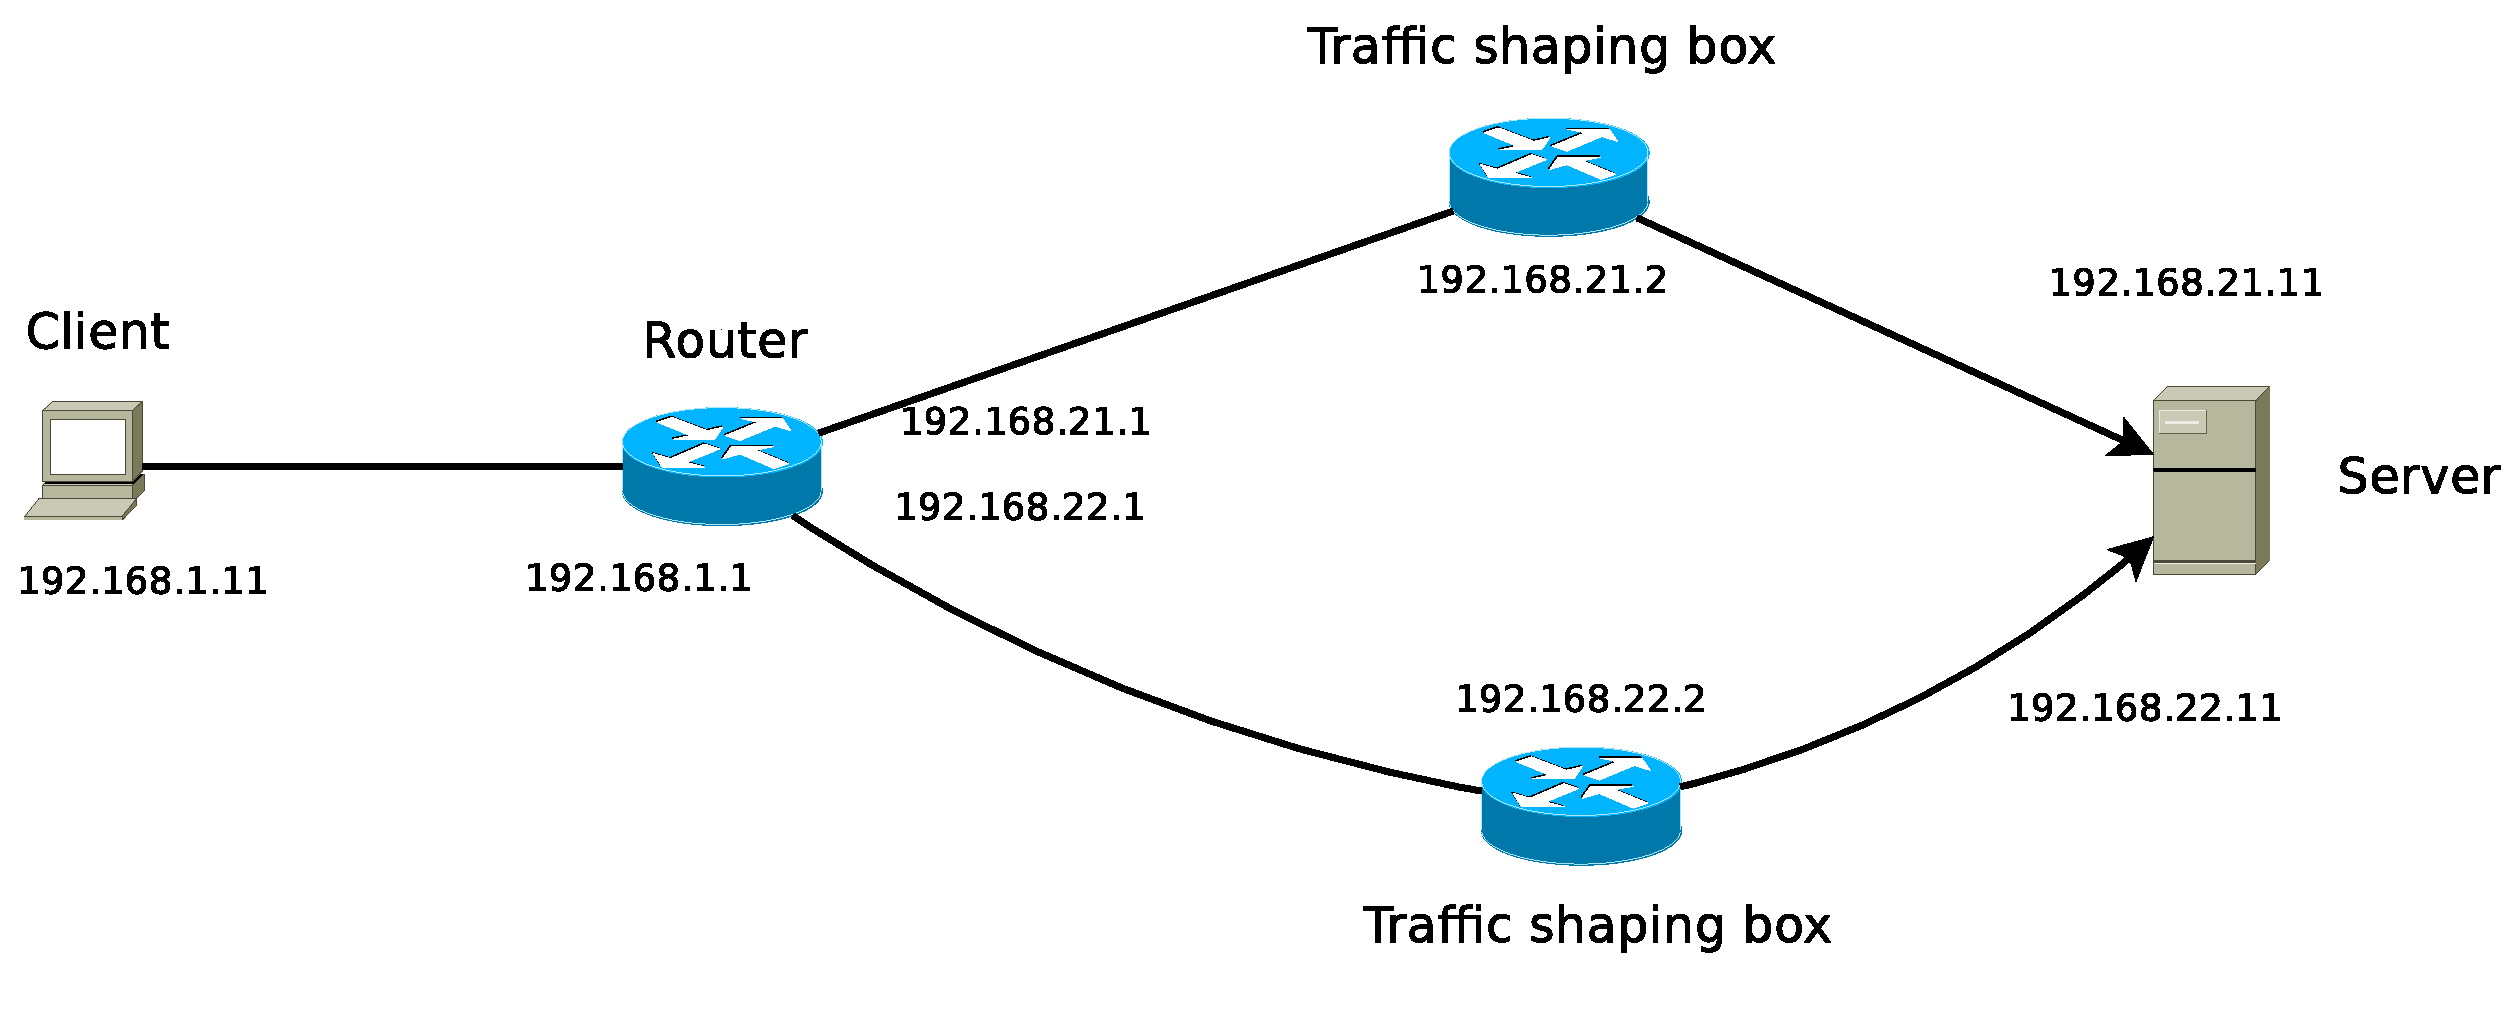
\includegraphics[width=12cm]{./images/setup.eps}
    \caption{Setup}
    \label{setup_fig}
  \end{figure}

  As show in figure ~\ref{setup_fig} the setup consists of five machines :

  \begin{itemize}
    \item One home computer, a client.
    \item One server for the OpenVPN server
    \item One home router connected to the OpenVPN server, by two ethernet cable to enable MPTCP to use two subflows.
    \item Two routers to do some traffic shaping.
  \end{itemize}

  \subsubsection{OpenVPN client}

  It is a TP-LINK N900 router, its CPU is a PPC P1014@800MHz and it has 128Mb of RAM \autocite{openwrt_n900}.
  It will be running OpenWRT with a custom kernel 3.10.49 with MPTCP v0.89.0-rc compiled by Sébastien Barré and Gregory Detal.

  \subsubsection{Traffic shaping boxes}
  The traffic shaping boxes will mainly limit the brandwith and add delay between the router and the server to emulate real internet connections speed.
  They are TP-Link TL-WR741ND router, CPU Atheros AR7240 @ 350 MHz and 32Mb of RAM. It will be running OpenWRT with tc, a shaping software, installed.

  \subsubsection{OpenVPN server}
  The OpenVPN server is a computer with a Intel Pentium 4 CPU and 2Go of RAM.
  It will be using debian running kernel 3.14.33 from the MPTCP Github repository \ref{mptcp} with MPTCP v0.89.5 compiled with all the TCP congestion algorithms.

  The client computer will connect to the router and access the server through it.

  For the purpose of these tests we decided not to use encryption or authentification on the OpenVPN tunnel, mainly because it need more CPU power and the TP-LINK N900 is not powerfull.
  Using encryption and authentification would have decrease performances and given that the main goal of this paper is not security, encryption is not needed.

  \subsection{OpenVPN configuration} \label{sec:openvpn_config}

  Listing~\ref{lst:openvpn_config_client} presents the important parameters in the OpenVPN configuration file. The whole configuration can be found in the annexes.

  \begin{lstlisting}[caption={Openvpn configuration},label={lst:openvpn_config_client}]
  auth none
  cipher none
  sndbuf 0
  rcvbuf 0\end{lstlisting}

  As \textit{auth} and \textit{cipher} are about encryption and anthentification, they are disable because, as explained earlier,
  they add more overhead to packet and are not needed for these tests because privacy is not our concern.

  \textit{sndbuf} and \textit{rcvbuf} are two very important settings that are used by OpenVPN to set the \textit{SO\_SNDBUF} and \textit{SO\_RCVBUF} options on individual socket with setsockopt.
  The \textit{SO\_SNDBUF} and \textit{SO\_RCVBUF} options are the send and receive buffer size.
  When they are set to 0, OpenVPN does not set value with setsockopt and the value from the OS are used.

  After reading quite a lot about these two parameters the most common advise for Linux is to use a value of 0 for \textit{sndbuf} and \textit{rcvbuf} because it let the
  OS taking care of adjusting the TCP window size.

  For the purpose of the tests in this paper, it is important to keep control on the size of the TCP window to be able to evaluate their impact.
  Consequently, I will set values for \textit{sndbuf} and \textit{rcvbuf} manually.

  The advantage of using these settings instead of set globally the value with the help of sysctl is that it only affect sockets created by OpenVPN and not all
  the sockets and it is easier to change.

  \subsection{Delay boxes}

  The two delay boxes are placed between the OpenWRT router and the server, one for each link. Their goal is to limit the bandwidth and introduce delay on links.

  For this I used tc, a traffic control tool in the linux kernel, used to configure and control the network schedulers. It enables to choose between a sets
  of queing systems and mechanisms to control how the packets are received and transmitted. This is usually called QoS (Quality of service).

  It gives the possibility to :
  \begin{itemize}
    \item Limit the total bandwidth of a link using TBF or HTB
    \item Give priority to latency sensitive traffic
    \item Distribute unreserved bandwidth equitably
    \item Reserve bandwidth for a particular application
    \item Limit the bandwidth of a particular user, service or client
    \item Introduce delay, loss, duplication, reordering (netem)
  \end{itemize}

  From the many possibilities offered by tc, I use in this paper the first and the last one, using TBF and netem.
  Here is an example :

  \begin{lstlisting}
    # tc qdisc add dev eth0 root handle 1:0 tbf rate 8mbit burst 50k latency 5ms
    # tc qdisc add dev eth0 parent 1:1 handle 10: netem delay 50ms
  \end{lstlisting}

  The first line of this script will add a \textit{qdisc} which is a scheduler to the interface \textit{eth0}. The handle is the name given for this \textit{qdisc} on the interface \textit{eth0}.
  The handle is defined by a number of form major\:minor, it is followed by a class type, tbf which is a queuing discipline to attach to the \textit{qdisc}.
  It will limit the rate to 8mbit and set the buffer to 50k.

  The second line add a class to the interface \textit{eth0} on the parent handle (from line 1). Again we give a handle and then we give the class type,
  netem. It will add a delay of 50ms to the interface \textit{eth0}.

  In this example we use netem to add delay to the link and then use TBF to add a bandwidth limit. This simple process is adequate to our needs.


    \begin{figure}[h!]
     \centering
     \includegraphics[width=8cm]{./images/tc.png}
     \captionsource{Token Bucket Filter}{\cite{stackoverflowtbf}}
     \label{fig_tbf}
    \end{figure}

    Figure \ref{fig_tbf} presents how TBF works in practice. The burst parameter is equivalent to the size of the bucket, it holds a limited amount of tokens and if
    too many are added the bucket overflows and the tokens are lost.

    The latency or limit is the number of packets that can sit into the line waiting to get a token.
    This occurs when the bucket is empty or if the bucket does not have enough tokens for all the packets.

    When the kernel send a packet it first needs to obtain a tokens.
    If it does not obtains a token it is put in a line to wait for a token and if this line is full it is dropped.

  \section{Tests Procedures}

  To mesure the differences in term of performance when using OpenVPN we will measure the throughput, the delay and the CPU usage using different configurations such as follow :

  \begin{enumerate}
    \item UDP protocol as OpenVPN protocol
    \item TCP protocol as OpenVPN protocol with MPTCP using 2 links (2 subflow)
  \end{enumerate}

  The tests will be ran using different link speed to mimic real internet connection speed.
  For that I looked for the different FAI in Belgium and listed their available speeds in April 2015.

  Here are the one selected for the tests :
  \begin{itemize}
    \item  8mbps (edpnet)
    \item  32mpbs (voo telenet)
    \item  100mbps (numericable)
  \end{itemize}

  Delay will also be introduces on the links to see how the performances may vary.
  \begin{itemize}
    \item  1ms
    \item  25ms
    \item  200ms
  \end{itemize}

  \subsection{Bulk data transfer}

  A common type of network traffic on the internet especially with the cloud is bulk data transfers.
  It is used when pulling files from a FTP or accessing data on your shared drive (google drive or dropbox).

  To simulate this type of traffic, I use the TCP\_MAERTS a test from Netperf, it measure bulk data transfer performance. This will measure how fast the server can send data to the client.

  \subsubsection{TCP\_MAERTS}

  TCP\_MAERTS test open a single TCP connection to the remote machine and makes as many rapid write calls as possible. These write calls have a specific size which by default is the sender buffer send size.

  The socket buffers on either end will be sized according to the systems default and all TCP options will be at their default settings.

  Options :
  \begin{itemize}
\item -s size Sets the local socket send and receive buffers (size in bytes)
\item -S size Sets the remote socket send and receive buffers (size in bytes)
\item -m size Sets the local send message size to size
\item -M size Sets the remote receive message size to size
\item -D Sets the TCP\_NODELAY socket option on both the local and
remote systems
  \end{itemize}

  \subsection{TCP Request/Response}  \label{sec:setup_request_response}

  Another common type of network traffic on the internet between client and server is the request/response model.
  This model is based on individual transactions between the client and the server.
  The client sends a request to the server, the server receives it, process it and sends a response back to the client.

  To mimic this type of traffic, the TCP\_CRR test from Netperf will be used.
  Apache Benchmark (AB) will also be used because the  TCP\_CRR is sequential and it is interesting to analyse the impact on the results when multiple connections are used at the same time.
  The server will have a Apache server with the default settings and will serve the default apache welcome page.

  \subsubsection{TCP\_CRR}

  TCP\_CRR measures the performances of establishing a connection, exchanging a single request/response transaction, and tearing-down that connection.
  This is similar to the process of an HTTP 1.0 or HTTP 1.1 connection when HTTP Keepalives are not used. It is a synchronous, one transaction at a time, request/response test.
  By default the message size is 1 byte but it can be changed using options.

  Options :
  \begin{itemize}
\item -r req,resp sets the size of the request or response message, or both
\item -s size sets the size of the local socket send and receive buffers to
size bytes
\item -S size sets the size of the remote socket send and receive buffers to
size bytes
\item -D sets the TCP\_NODELAY socket option on both the local and
remote system
  \end{itemize}

    \subsubsection{Apache Benchmark (AB)}
    Apache Benchmark (AB) is a tool for benchmarking HTTP server. It shows how many request per second the server can deliver to the client by sending a arbitrary number of concurrent request.
    It has been created to benchmark the Apache web server.

    \section{Git Repository}

    To make all the tests reproductable, I have try to automize as much as possible, using mainly python and bash script.
    Everything is avaible on a git repository on Github \url{https://github.com/alokhan/memoire}.

    In this repository you find all the configuration files used for the router and server, all the script used to generate the graphics,
    ,all the \textit{.csv} files containing the test results used for this paper and also some documentation.
